\documentclass[border=10pt]{standalone}
\usepackage[svgnames]{xcolor}
\usepackage{amsmath}
\usepackage{pgfplots}
\pgfplotsset{compat=newest}
\usepackage[sfdefault]{FiraSans}
\usepackage{FiraMono}
\renewcommand*\familydefault{\sfdefault}
\begin{document}
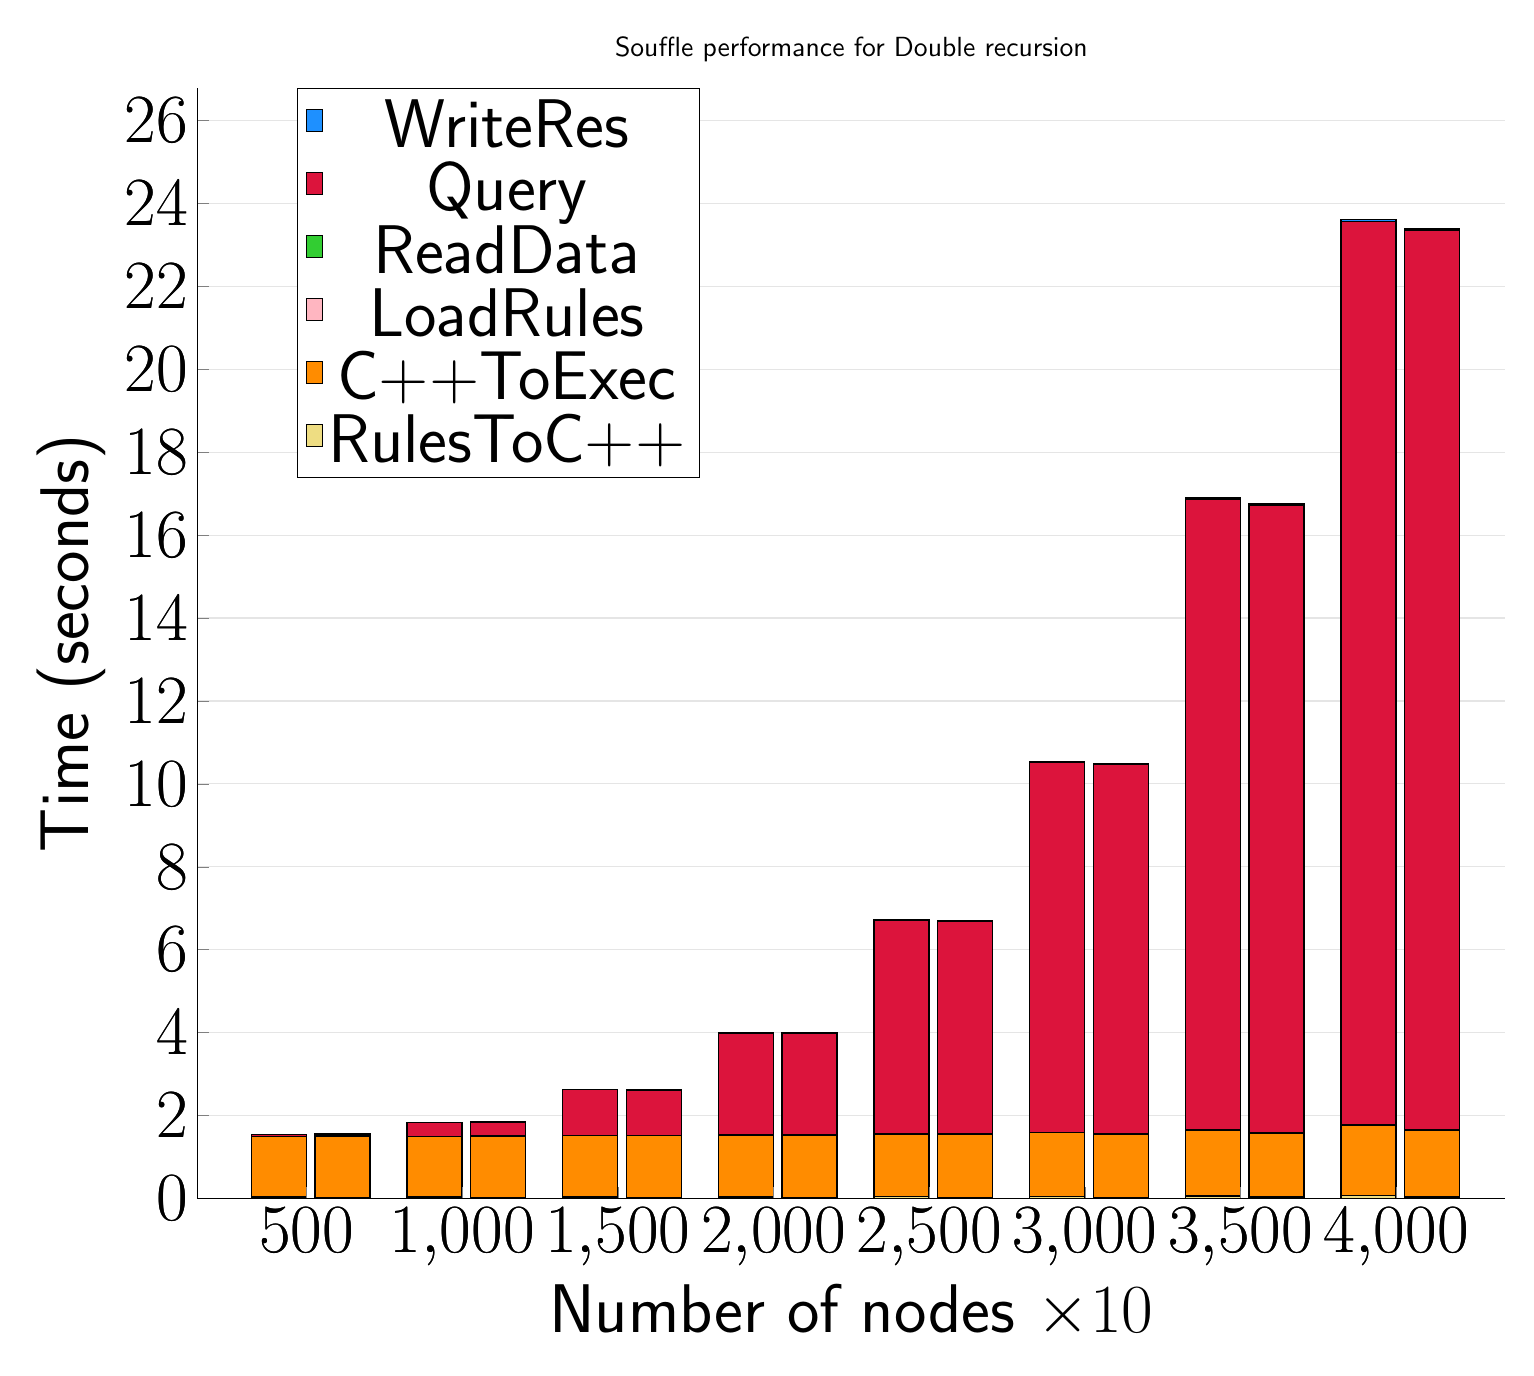
\begin{tikzpicture}
\begin{axis}[
   ybar stacked,
   title={Souffle performance for Double recursion},
   bar shift=-10pt,
   width=1.5\textwidth,
   bar width=0.7cm,
   ymajorgrids, tick align=inside,
   major grid style={draw=gray!20},
   xtick=data,
   ymin=0, ymax=26.78465,
   axis x line*=bottom,
   axis y line*=left,
   enlarge x limits=0.1,
   legend style={
       at={(0.23, 1)},
       anchor=north,
       legend columns=1,
       font=\Huge,
   },
   ylabel={Time (seconds)},
   xlabel={Number of nodes $\times 10$},
   label style={font=\Huge},
   tick label style={font=\Huge},
]
\addlegendimage{fill=DodgerBlue, draw=black, line width=0.2pt}
\addlegendentry{WriteRes}
\addlegendimage{fill=Crimson, draw=black, line width=0.2pt}
\addlegendentry{Query}
\addlegendimage{fill=LimeGreen, draw=black, line width=0.2pt}
\addlegendentry{ReadData}
\addlegendimage{fill=LightPink, draw=black, line width=0.2pt}
\addlegendentry{LoadRules}
\addlegendimage{fill=DarkOrange, draw=black, line width=0.2pt}
\addlegendentry{C++ToExec}
\addlegendimage{fill=LightGoldenrod, draw=black, line width=0.2pt}
\addlegendentry{RulesToC++}
\addplot +[fill=LightGoldenrod, draw=black, line width=0.5pt] coordinates {
    (500, 0.04000000953674317)
    (1000, 0.04000005722045898)
    (1500, 0.040999984741210936)
    (2000, 0.04100000858306885)
    (2500, 0.04400002956390381)
    (3000, 0.04499998092651367)
    (3500, 0.060999941825866696)
    (4000, 0.07900004386901856)
};
\addplot +[fill=DarkOrange, draw=black, line width=0.5pt] coordinates {
    (500, 1.4539999961853027)
    (1000, 1.4579999446868896)
    (1500, 1.4830000162124635)
    (2000, 1.4880000114440919)
    (2500, 1.5149999856948853)
    (3000, 1.5450000047683716)
    (3500, 1.5910000324249267)
    (4000, 1.6869999885559082)
};
\addplot +[fill=LightPink, draw=black, line width=0.5pt] coordinates {
    (500, 9.66127e-05)
    (1000, 8.70667e-05)
    (1500, 6.6821e-05)
    (2000, 3.34709e-05)
    (2500, 5.25083e-05)
    (3000, 0.00010956660000000002)
    (3500, 9.86417e-05)
    (4000, 7.494159999999999e-05)
};
\addplot +[fill=LimeGreen, draw=black, line width=0.5pt] coordinates {
    (500, 0.001464262)
    (1000, 0.002620666)
    (1500, 0.0035486829999999995)
    (2000, 0.0044367090000000005)
    (2500, 0.005588308)
    (3000, 0.006691643999999999)
    (3500, 0.008360300000000001)
    (4000, 0.008500437)
};
\addplot +[fill=Crimson, draw=black, line width=0.5pt] coordinates {
    (500, 0.05367539)
    (1000, 0.3313687)
    (1500, 1.09908)
    (2000, 2.4580069999999994)
    (2500, 5.145857000000001)
    (3000, 8.923101999999998)
    (3500, 15.202070000000003)
    (4000, 21.78465)
};
\addplot +[fill=DodgerBlue, draw=black, line width=0.5pt] coordinates {
    (500, 0.0009775329)
    (1000, 0.002977619)
    (1500, 0.00656182)
    (2000, 0.01149457)
    (2500, 0.017667429999999998)
    (3000, 0.025839690000000005)
    (3500, 0.035073999999999994)
    (4000, 0.04558554)
};
\end{axis}
\begin{axis}[
   ybar stacked,
   bar shift=13pt,
   width=1.5\textwidth,
   bar width=0.7cm,
   ymajorgrids, tick align=inside,
   major grid style={draw=none},
   xtick=data,
   ymin=0, ymax=26.78465,
   axis x line*=none,
   axis y line*=none,
   enlarge x limits=0.1,
   label style={font=\Huge},
   tick label style={font=\Huge},
]
\addplot +[fill=LightGoldenrod, draw=black, line width=0.5pt] coordinates {
    (500, 0.030000000000000006)
    (1000, 0.030000000000000006)
    (1500, 0.030000000000000006)
    (2000, 0.030000000000000006)
    (2500, 0.031000000000000007)
    (3000, 0.031000000000000007)
    (3500, 0.036)
    (4000, 0.041999999999999996)
};
\addplot +[fill=DarkOrange, draw=black, line width=0.5pt] coordinates {
    (500, 1.473)
    (1000, 1.4760000000000002)
    (1500, 1.4920000000000002)
    (2000, 1.504)
    (2500, 1.5240000000000002)
    (3000, 1.525)
    (3500, 1.539)
    (4000, 1.605)
};
\addplot +[fill=LightPink, draw=black, line width=0.5pt] coordinates {
    (500, 9.609999999999999e-05)
    (1000, 8.65e-05)
    (1500, 6.63e-05)
    (2000, 3.33e-05)
    (2500, 5.22e-05)
    (3000, 0.0001088)
    (3500, 9.77e-05)
    (4000, 6.45e-05)
};
\addplot +[fill=LimeGreen, draw=black, line width=0.5pt] coordinates {
    (500, 0.0014632)
    (1000, 0.0026191)
    (1500, 0.0035453)
    (2000, 0.0044359)
    (2500, 0.005587399999999999)
    (3000, 0.0064504)
    (3500, 0.0079138)
    (4000, 0.008193200000000001)
};
\addplot +[fill=Crimson, draw=black, line width=0.5pt] coordinates {
    (500, 0.0535867)
    (1000, 0.3307171)
    (1500, 1.095862)
    (2000, 2.450427)
    (2500, 5.131427)
    (3000, 8.899659)
    (3500, 15.14585)
    (4000, 21.698890000000002)
};
\addplot +[fill=DodgerBlue, draw=black, line width=0.5pt] coordinates {
    (500, 0.0009061)
    (1000, 0.0029717)
    (1500, 0.0065487)
    (2000, 0.011430899999999999)
    (2500, 0.017599999999999998)
    (3000, 0.025351999999999996)
    (3500, 0.034351900000000005)
    (4000, 0.04497399999999999)
};
\end{axis}
\end{tikzpicture}

\end{document}
